\documentclass[mathserif,12pt]{beamer}
% \usepackage[size=custom,width=77,height=107,scale=1.4,orientation=portrait]{beamerposter} 

% option "t" means align top
% option "handout" for handout mode (each frame takes only one page)
% option "notes" to add notes pages

\mode<presentation>
{
  \usetheme{bo-poster}
}
\usepackage[size=custom,width=12,height=1.5,scale=0.2,orientation=portrait]{beamerposter}

\title{\LARGE\textbf{Surrogate Regret Bounds for Polyhedral Losses}\vspace*{-5pt}}
%\titlegraphic{
%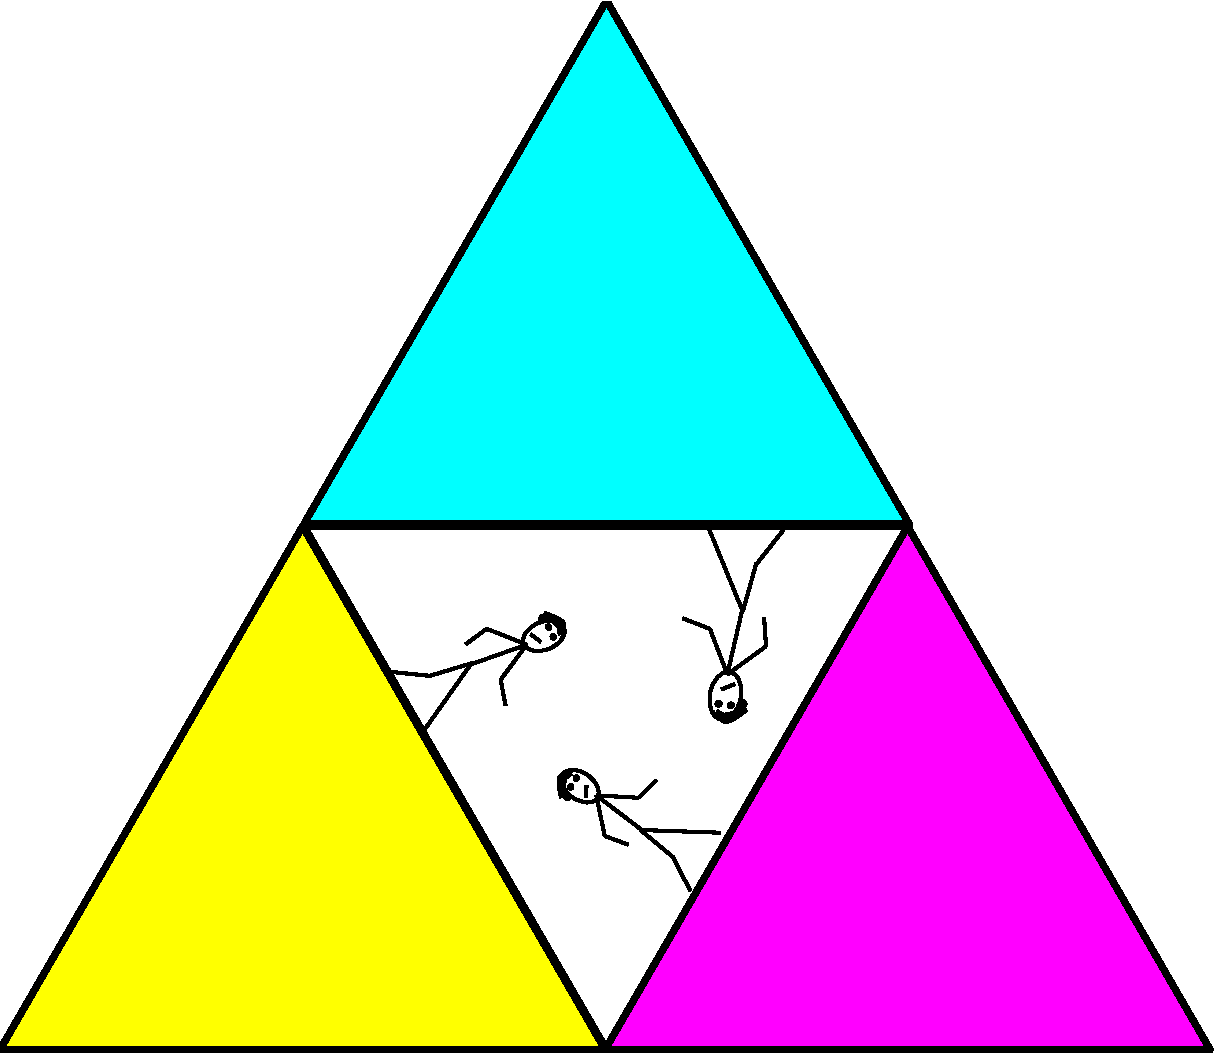
\includegraphics[width=.35\textheight]{figs/logo}
%}

\author{{\large\textbf{Rafael Frongillo} and \textbf{Bo Waggoner}} \and {\large University of Colorado, Boulder}}
\date{\large\textbf{NeurIPS 2021}}

\begin{document}

% \titlepage

\begin{frame}{}
  \vspace*{-15pt}
  
  \begin{beamercolorbox}{block title}
    \smallskip
    
    \textbf{\hfill \LARGE Surrogate Regret Bounds for Polyhedral Losses \hfill}
    \smallskip
  \end{beamercolorbox}

  \smallskip
  \hfill
  {\large\textbf{Rafael Frongillo} and \textbf{Bo Waggoner}}
  \hspace{20pt}
  {\large University of Colorado, Boulder}
  \hfill
  {\large \textbf{NeurIPS 2021}}
  \hfill~
  
  \vspace*{-30pt}
  
\end{frame}

\end{document}


%%% Local Variables:
%%% mode: latex
%%% TeX-master: t
%%% End:
